\documentclass[11pt]{article}
\usepackage[margin=1in]{geometry}
\usepackage[numbers,sort&compress]{natbib}
\usepackage{amsmath,amssymb}
\usepackage{booktabs}
\usepackage{graphicx}
\usepackage{tikz}
\usetikzlibrary{arrows.meta,positioning,calc}
\usepackage[hidelinks]{hyperref}
\usepackage{xcolor}
\usepackage{microtype}

\newcommand{\psilm}{$\Psi$LM}
\newcommand{\code}[1]{\texttt{#1}}

\title{\psilm: Coupling Frozen Language and Physics Models\\through Trainable Latent Bridges}

\author{Ryoji Furui\thanks{\url{https://github.com/ryoji-info/PsiLM}. \textbf{AI generation disclosure:} the research reported here was designed, implemented, executed, and written up by \emph{Claude Fable 5} (Anthropic), working autonomously on the author's Apple M2 laptop under the author's direction; see Section~\ref{sec:disclosure}.}}
\date{August 30, 2026}

\begin{document}
\maketitle

\begin{abstract}
We ask whether a pretrained language model and a pretrained physics model can run as one system --- two frozen networks answering a single question with communication carried entirely by hidden states, the way the brain's hemispheres cooperate across the corpus callosum. As of August 2026 we find no published work coupling a pretrained LLM to a neural-operator physics model through a bidirectional latent channel at inference. We build such a system, \psilm{}, on a consumer laptop (Apple M2, 24\,GB), in four steps. (1) Tool-loop baselines reproduce the known capability-gap effect: a simulator adds $+28.3$ points to a 3B model on physics QA but \emph{hurts} a 0.5B model. (2) We produce, to our knowledge, the first public reproduction of the Bicameral Model \citep{flamant2026bicameral}: two frozen Qwen2.5-0.5B streams coupled by a 6.2M-parameter gated hidden-state interface reproduce the paper's phase transition, reaching 100\% exact tool recall through the latent channel alone. (3) With the auxiliary language model replaced by a frozen Fourier Neural Operator, \psilm{} answers Burgers-equation field-value questions at 100\% (tolerance $\pm 0.05$; MAE 0.014) where the LLM alone achieves 5\%, matching the accuracy of an oracle that states the answer in text --- with no text at the interface. (4) The result survives hardening: held-out question families expose a clean generalization law (\emph{support coverage} --- readouts generalize only where their training support covers the test distribution, a hypothesis we confirm by refuting the alternative), and the architecture transfers to 2D reaction--diffusion with a pretrained physics foundation model (DPOT-Tiny) as the hemisphere, scoring 95\%, within five points of the oracle ceiling. All experiments, including two failed designs and one refuted hypothesis, are reproducible from the public repository on a single consumer machine.
\end{abstract}

\section{Introduction}
\label{sec:intro}

Large language models reason in discrete tokens; physics foundation models \citep{barman2025lpm,hao2024dpot} evolve continuous fields. The human brain suggests a third architecture: specialized regions, neither subordinate to the other, co-processing a single task through dense internal communication. This paper takes the analogy literally. We couple a frozen pretrained LLM to a frozen pretrained physics model through small trainable \emph{bridges} operating purely on hidden states --- the language stream never sees the physics as text, and the physics model never parses a sentence --- and ask whether the coupled system can answer questions neither component can answer alone.

A second motivation is epistemic. In the wave--particle picture of quantum mechanics, a discrete observation is one reading of an underlying continuous process; Bohr called the two descriptions \emph{complementary}. \psilm{} instantiates that structure operationally: a continuous field evolved by a neural operator, and a discrete verbal reading of it produced by a language model, with a learned interface deciding what crosses between them. The name is the wave function $\Psi$.

Our literature survey (Section~\ref{sec:related}) found the ingredients of such a system published separately --- frozen-model latent bridges \citep{bansal2024calm,zolna2024gats}, two LLMs coupled in hidden-state lockstep \citep{flamant2026bicameral}, LLM--simulator loops through text \citep{liu2023mindseye,varambally2026zephyrus}, and brain-inspired shared workspaces \citep{vanrullen2021glw,goyal2022workspace} --- but no published coupling of a pretrained LLM to a neural-operator physics model through a bidirectional latent channel at inference, a gap independently noted as open by a survey of latent inter-model communication \citep{liu2026beyondtokens}. We fill it at small scale, on consumer hardware, with the following contributions:

\begin{enumerate}
\item \textbf{Baselines} (Sec.~\ref{sec:stage0}): a seeded physics-QA benchmark on which text-level tool coupling reproduces the published capability-gap effect ($+28.3$ points at 3B, $-3.3$ at 0.5B).
\item \textbf{A reproduction} (Sec.~\ref{sec:stage1}): the first public reimplementation of the Bicameral Model \citep{flamant2026bicameral}, confirming its training phase transition and its causal order, and documenting two facts the paper does not: an inference bootstrap required at the uncoupled prompt boundary, and a teacher-forced/rollout dissociation showing exposure bias dominates evaluation at this scale.
\item \textbf{\psilm{}} (Sec.~\ref{sec:psilm}): a frozen LLM and a frozen neural operator coupled through $\sim$3.5M trainable bridge parameters, reaching the oracle-text ceiling on 1D Burgers field-value QA (100\% vs.\ 5\% for the LLM alone).
\item \textbf{A generalization law} (Sec.~\ref{sec:gen}): on held-out question families the interface transfers partially, failure is attributable to a single readout, and a controlled experiment refutes the natural ``classify, don't regress'' fix --- establishing \emph{support coverage} as the operative principle.
\item \textbf{Foundation-model transfer} (Sec.~\ref{sec:2d}): the architecture carries to 2D reaction--diffusion with pretrained DPOT-Tiny \citep{hao2024dpot} as the physics hemisphere (95\% vs.\ 6.7\% alone).
\end{enumerate}

\section{Related Work}
\label{sec:related}

\textbf{Text- and tool-level coupling.} Mind's Eye \citep{liu2023mindseye} pioneered LLM reasoning grounded by a physics engine through prompt round-trips; RAP \citep{hao2023rap} framed reasoning as an agent conversing with a world model in text; Zephyrus \citep{varambally2026zephyrus} couples an LLM to numerical weather foundation models through code; SGA \citep{ma2024sga} alternates an LLM with differentiable simulation for scientific discovery; RIA \citep{sun2026ria} closes an LLM/world-model loop per decision step for driving. In all of these the physics side is a subroutine reached through text or code. Multiagent debate \citep{du2024debate} couples multiple reasoner instances through exchanged messages; Cicero \citep{bakhtin2022cicero} combines a language model with a strategic-reasoning module through structured intents. Position papers argue that language, agent, and world models must interoperate \citep{hu2023law,lecun2022ami}.

\textbf{Latent-level coupling.} Flamingo \citep{alayrac2022flamingo} and BLIP-2 \citep{li2023blip2} graft frozen perception onto frozen LLMs unidirectionally; CALM \citep{bansal2024calm} cross-attends between two frozen LLMs' layers; GATS \citep{zolna2024gats} exchanges activations bidirectionally among frozen models at different rates. Socratic Models \citep{zeng2023socratic} made language itself the inter-model protocol; a fast-moving line replaces it with embeddings, activations, or KV state \citep{pham2024cipher,ramesh2025activations,zou2025latentmas,liu2026wormhole,shen2024collm,rodionov2025hogwild,wang2025parallelsurvey}; DroidSpeak \citep{liu2024droidspeak} shows even same-architecture models need repair to share raw state, motivating trained interfaces. Closest to our Stage~1, the Bicameral Model \citep{flamant2026bicameral} runs two frozen LLMs in per-token lockstep through a trainable gated interface; no code was released.

\textbf{Brain-inspired modular systems.} The Global Workspace line \citep{vanrullen2021glw,devillers2023gw,maytie2025gwdreamer,goyal2022workspace} couples frozen specialists through a learned shared latent space; bilateral architectures \citep{rajagopalan2022bilateral,rinaldo2024leftright} build literal two-hemisphere networks with an ablated callosal channel; \citet{bena2024specialization} show module specialization requires a bandwidth-constrained channel. Dual-process agents \citep{booch2021sofai,deepmind2024talker} and dual-system robot policies \citep{figure2025helix,nvidia2025groot} run a slow semantic model and a fast control model concurrently over latent interfaces.

\textbf{Language and PDE operators.} UPS \citep{shen2024ups} projects FNO features into a pretrained LLM's token space; Unisolver \citep{zhou2025unisolver} conditions a neural solver on frozen-LLM equation embeddings; ICON-LM \citep{yang2025iconlm} fine-tunes a GPT-2 into an operator learner; Text2PDE \citep{zhou2025text2pde} generates rollouts from text; \citet{negrini2025multimodalpde} decode operator states into text within one purpose-trained network. Each realizes one direction, or fuses everything into a single network; none couples two \emph{pretrained} models bidirectionally at inference.

\section{Experimental Platform}
All experiments run on one Apple M2 laptop with 24\,GB unified memory. The language hemisphere is frozen Qwen2.5-0.5B-Instruct \citep{qwen2025qwen25} (hereafter Qwen2.5-0.5B; fp16 on PyTorch MPS; 4-bit MLX quantizations for Stage~0), staged so a forward pass can pause at any decoder layer, exchange state, and resume; the staged pass is bit-exact against the stock model. Ground truth for the PDE tasks (Sections~\ref{sec:psilm}--\ref{sec:2d}) comes from spectral solvers with integrating-factor RK4 (dt-convergence $\le 4\times10^{-11}$; analytic limits verified), never from the neural physics models; Stages 0--1 are scored against closed-form mechanics and exact arithmetic. Trained components are only the interfaces (2--7M parameters); training runs in resumable 1000-step chunks at 2.2--4.0\,s/step.

\section{Stage 0: Text-Level Tool Coupling}
\label{sec:stage0}
We construct a seeded 60-item benchmark of rigid-body comparison questions (five scene types; one third are physics traps such as equal-mass free fall and complementary launch angles) scored against closed-form mechanics, and evaluate an \emph{alone} arm against a \emph{tool} arm in which the LLM extracts scene parameters as JSON, a simulator computes the outcome, and the result returns to the prompt \citep{liu2023mindseye}. Parameter extraction succeeds on 100\% of items at both model sizes, yet coupling helps only the larger model: Qwen2.5-3B improves $38.3\%\!\to\!66.7\%$ ($+28.3$, matching Mind's Eye's published $+27.9$ zero-shot average), while Qwen2.5-0.5B \emph{degrades} $35.0\%\!\to\!31.7\%$ --- it cannot reliably compare two numbers handed to it in text. Evidence \emph{use}, not extraction, is the bottleneck, motivating a trained interface that delivers evidence below the token level.

\section{Stage 1: Reproducing the Bicameral Model}
\label{sec:stage1}

We reimplement the Bicameral Model \citep{flamant2026bicameral} from its published specification: two frozen Qwen2.5-0.5B streams generate in lockstep; a trainable interface reads the primary's residual stream at layer 10 and writes a gated update into the auxiliary at layer 10 (forward coupling), and symmetrically auxiliary$\to$primary at layer 15 (reverse), each update $h \leftarrow (1-\sigma)h + \sigma f(h_{\text{send}})$ with the suppression gate $\sigma$ computed from the \emph{receiver}. The auxiliary drives a calculator whose output is forced into the auxiliary stream only; the primary receives results exclusively through the latent channel. We train the 6.2M-parameter interface with dual-target SFT on procedurally generated multiplication with causality-aligned auxiliary traces (192k samples).

\begin{figure}[t]
\centering
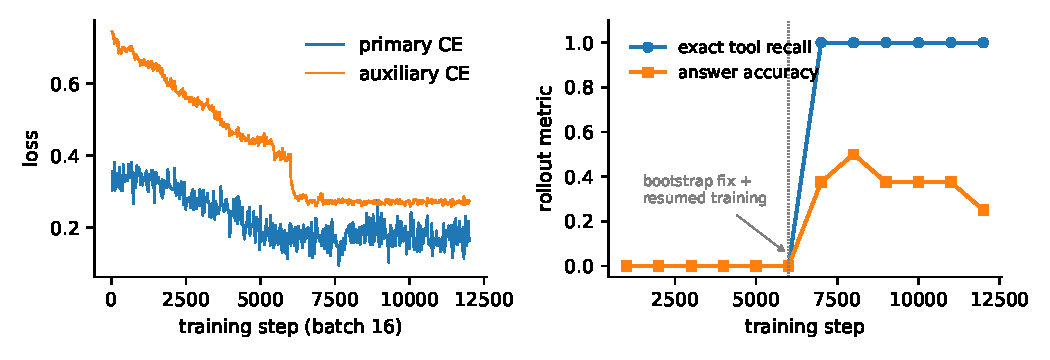
\includegraphics[width=\linewidth]{figs/stage1.pdf}
\caption{Stage 1 reproduction. \textbf{Left:} teacher-forced losses. \textbf{Right:} rollout metrics per 1000-step chunk. Exact tool recall undergoes the paper's phase transition ($0\!\to\!1.00$ within one chunk, at $\sim$112k samples) after an inference-bootstrap fix at step 6000; answer accuracy sets in after recall, in the paper's causal order.}
\label{fig:stage1}
\end{figure}

\textbf{The phase transition reproduces, in its causal order} (Fig.~\ref{fig:stage1}): forward coupling strengthens first, exact tool recall then jumps $0.00\!\to\!1.00$ in a single chunk, and answer accuracy sets in afterward. On held-out problems (7--10-digit products) the coupled system emits the exact \code{calc(A*B)} on 100\% of rollouts --- the auxiliary reads the operands entirely from hidden states --- while the reverse channel carries the leading 4--6 result digits reliably and degrades toward the tail (digit similarity 0.689 vs.\ 0.371 for the frozen model alone; exact match only 2.5\% at this length, $\sim$25--50\% on the shorter mixed-length products of the per-chunk rollout evaluations, $n{=}8$ each).

Two findings absent from the original paper: (i) the first auxiliary token is predicted from the \emph{uncoupled} prompt tail, a position training can never influence, so free-running generation derails without a protocol-level bootstrap (we force two initial wait tokens); (ii) high teacher-forced channel quality coexists with zero rollout success until that bootstrap exists --- exposure bias dominates evaluation at this scale (the committed diagnostic at the final checkpoint, \code{teacher\_forced\_diagnostic.json}: 100\% call-token accuracy and 63.0\% per-digit, against 0\% rollouts before the bootstrap).

\section{\psilm{}: A Language Model Coupled to a Neural Operator}
\label{sec:psilm}

\begin{figure}[t]
\centering
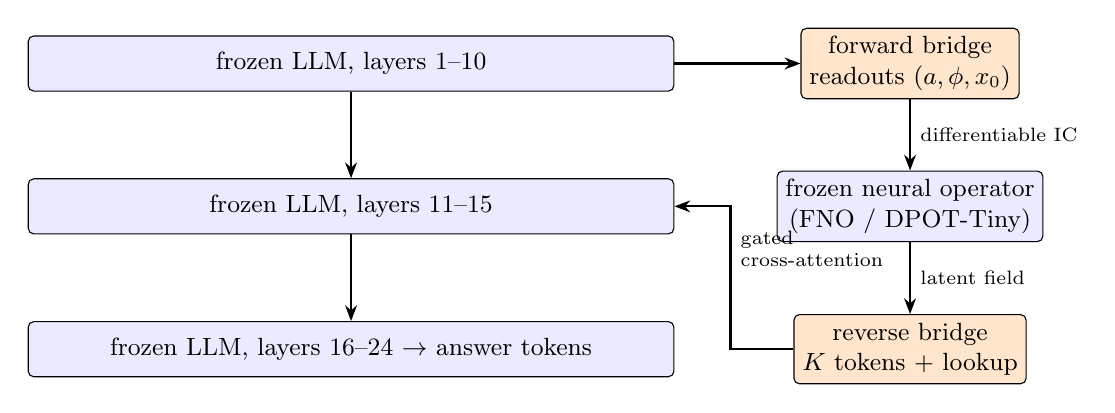
\begin{tikzpicture}[font=\small, node distance=4mm,
  box/.style={draw, rounded corners=2pt, minimum height=7mm, inner sep=3pt},
  frozen/.style={box, fill=blue!8},
  train/.style={box, fill=orange!20},
  arr/.style={-{Stealth[length=2mm]}, thick}]
\node[frozen, minimum width=82mm] (l10) {frozen LLM, layers 1--10};
\node[frozen, minimum width=82mm, below=11mm of l10] (l15) {frozen LLM, layers 11--15};
\node[frozen, minimum width=82mm, below=11mm of l15] (l24) {frozen LLM, layers 16--24 $\rightarrow$ answer tokens};
\node[train, right=16mm of l10.east, align=center, anchor=west] (fwd) {forward bridge\\readouts $(a,\phi,x_0)$};
\node[frozen, align=center] (fno) at (fwd |- l15) {frozen neural operator\\(FNO / DPOT-Tiny)};
\node[train, align=center] (rev) at (fwd |- l24) {reverse bridge\\$K$ tokens + lookup};
\draw[arr] (l10.east) -- (fwd.west);
\draw[arr] (fwd) -- (fno) node[midway, right, font=\scriptsize]{differentiable IC};
\draw[arr] (fno) -- (rev) node[midway, right, font=\scriptsize]{latent field};
\draw[arr] (rev.west) -- ++(-8mm,0) |- (l15.east) node[pos=0.35, right, font=\scriptsize, align=left]{gated\\cross-attention};
\draw[arr] (l10) -- (l15);
\draw[arr] (l15) -- (l24);
\end{tikzpicture}
\caption{\psilm{}. Orange components (3.5--3.7M parameters) are the only trained ones. The question is read out of the LLM's layer-10 hidden states; the frozen operator evolves the field; the result returns through a position-lookup token and gated cross-attention at layer 15. No text crosses the interface.}
\label{fig:arch}
\end{figure}

Stage 2 replaces the auxiliary language model with a genuine physics model (Fig.~\ref{fig:arch}). The task: ``$u(x,0)=a\sin(2\pi x+\phi)$ evolves by Burgers' equation ($\nu=0.02$) until $t=0.5$; what is $u$ at $x_0$?'' --- answered to two decimals, scored within $\pm 0.05$ on fields spanning $\pm 0.6$ (a degenerate always-zero strategy scores 7.9\% on the training distribution and 1.7\% on the held-out set of Table~\ref{tab:main}). The physics hemisphere is a 70K-parameter FNO trained once on solver data to $0.28\%$ relative error (one-shot $u_0 \mapsto u(\cdot,T)$, in the full-rollout style of contemporary physics foundation models) and then frozen.

\textbf{Forward bridge (language$\to$physics).} Learned queries attention-pool the LLM's layer-10 prompt states; heads regress $(a,\sin\phi,\cos\phi)$ and read the query position $x_0$ as a 100-way classification whose softmax expectation is differentiable and sharp. A differentiable sinusoid built from the readout feeds the operator, so answer-loss gradients flow from the LLM's words into the physics input.

\textbf{Reverse bridge (physics$\to$language).} $K{=}16$ learned queries compress the operator's latent field (plus Fourier positional features and the predicted field itself) into soft tokens, joined by a \emph{position-lookup token}: a periodic von Mises kernel of learnable sharpness, centered at the $x_0$ readout, samples the field ``where the question asked,'' with an auxiliary head deep-supervised on $u(x_0)$. All tokens enter the primary at layer 15 through gated cross-attention (receiver-computed suppression gate, near-closed initialization).

\textbf{Training} minimizes answer cross-entropy plus auxiliary readout losses (parameter MSE, $x_0$ CE, lookup-value MSE); both backbone networks stay frozen. Two design elements were forced by failure analysis, which we report as results: plain cross-attention over field summaries mode-collapsed to per-trajectory constants (the system answered the field's \emph{average} for every $x_0$), and a regressed $x_0$ (RMS error 0.06) was too blurry beside a shock; the classification pointer and the deep-supervised lookup cracked both: first-chunk rollout accuracy was 0.08 for both failed designs, then 0.50 and 1.00 in the final design's first two 16k-sample chunks (Fig.~\ref{fig:chunks} shows the final configurations).

\begin{table}[t]
\centering
\caption{Held-out results. Left: 1D Burgers ($n{=}60$). Right: 2D Fisher--KPP with pretrained DPOT-Tiny ($n{=}60$). Tolerance $\pm0.05$; greedy decoding; all arms share the frozen Qwen2.5-0.5B.}
\label{tab:main}
\small
\begin{tabular}{lrr@{\hspace{8mm}}rr}
\toprule
 & \multicolumn{2}{c}{1D Burgers (FNO)} & \multicolumn{2}{c}{2D Fisher--KPP (DPOT-Tiny)} \\
arm & acc@0.05 & MAE & acc@0.05 & MAE \\
\midrule
LLM alone & 5.0\% & 0.729 & 6.7\% & 0.337 \\
LLM + answer in text (oracle) & 100\% & 0.0028 & 100\% & 0.0024 \\
\textbf{\psilm{} (latent coupling)} & \textbf{100\%} & \textbf{0.0138} & \textbf{95.0\%} & \textbf{0.0168} \\
degenerate always-0.00 & 1.7\% & 0.308 & 1.7\% & 0.673 \\
\bottomrule
\end{tabular}
\end{table}

\textbf{Result} (Table~\ref{tab:main}, left): \psilm{} answers 100\% of held-out questions within tolerance (MAE 0.0138), matching the accuracy of an oracle that states the true value in the prompt --- while the frozen LLM alone scores 5\%. The answer travels entirely through hidden states: question out of the residual stream, simulation in the operator, value back through gated attention, verbalized by a frozen model.

\begin{figure}[t]
\centering
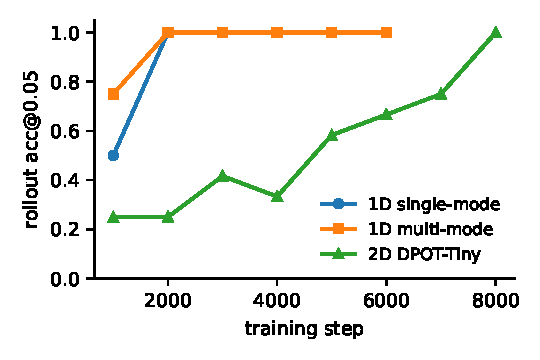
\includegraphics[width=0.48\linewidth]{figs/stage2_chunks.pdf}\hfill
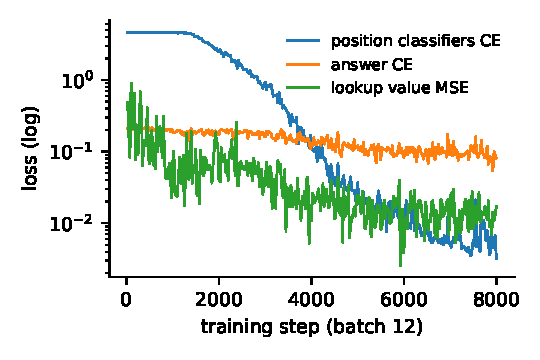
\includegraphics[width=0.48\linewidth]{figs/stage2d_phases.pdf}
\caption{\textbf{Left:} rollout accuracy per training chunk for the three \psilm{} configurations. \textbf{Right:} 2D training phase structure --- the four positional classifiers lock in first (over $\sim$5k steps); the answer loss converges only after the pointer does, echoing Stage~1's causal ordering.}
\label{fig:chunks}
\end{figure}

\section{Generalization: the Support-Coverage Law}
\label{sec:gen}

To harden the result we extend the initial conditions (ICs) to sums of sinusoids and train the bridges \emph{only on single-mode questions}, evaluating on three families: in-distribution, the held-out combination (two-term questions never seen), and amplitude extrapolation beyond the training range. The physics FNO is trained on a broader distribution than any evaluation family, so transfer failures are attributable to the interface. Results ($n{=}48$ per family): in-distribution 97.9\% (MAE 0.009); unseen combination 31.3\% (0.128); extrapolation 50.0\% (0.096) --- all above the LLM-alone (0--6.3\%) and always-zero (27.1\%, 16.7\%, 4.2\%) baselines, decisively so except against the combination family's zero baseline, and all far below in-distribution.

Teacher-forced attribution is unambiguous: the $x_0$ pointer generalizes \emph{perfectly} to every family (absolute error $\le 10^{-4}$), while the amplitude readout alone degrades $0.043 \to 0.355$ (combination) and $0.206$ (extrapolation); the record is committed as \code{attribution.json}. The natural hypothesis --- the classified quantity transfers, so classify the amplitudes too --- we tested with a v2 interface (per-mode pooling queries; amplitudes as 121-bin classifications). \textbf{It was worse on every family} (extrapolation $50\%\!\to\!19\%$, combination $31\%\!\to\!21\%$; v2 was evaluated at its 64k-sample convergence plateau --- rollout accuracy flat across its final two chunks --- vs.\ v1's 96k). The refutation identifies the real principle: $x_0$ generalized because all 100 of its bins occur in training, whereas amplitude bins outside the trained range never receive gradient and cannot move, while regression at least drifts. We summarize this as a \emph{support-coverage law}: a trained latent interface generalizes like a learned model, not a program --- coverage of the readout's support at training time, not the readout's parameterization, is what buys transfer. Section~\ref{sec:2d} applies the law prospectively.

\section{2D Physics with a Pretrained Foundation Model}
\label{sec:2d}

Finally we replace our own operator with DPOT-Tiny \citep{hao2024dpot}: a 7.5M-parameter AFNO operator pretrained across twelve PDE datasets, loaded with \code{strict=True} from the published checkpoint, fine-tuned for 1200 steps ($\approx$5 minutes) to 1.64\% relative error on our task, then frozen. The task moves to 2D Fisher--KPP reaction--diffusion on the periodic unit square: a Gaussian bump --- height, center, and width all stated in the question --- grows and spreads by $u_t = D\nabla^2 u + r\,u(1-u)$, and the question asks for $u$ at a point $(x_0,y_0)$ sampled within the front's active zone (always-zero scores 4.8\% on the training distribution; 1.7\% held-out). The IC is replicated across DPOT's 10-timestep input history; the reverse bridge attends over DPOT's 256 latent patch tokens plus a separable 2D periodic lookup on the predicted field; applying the support-coverage law, we make every positional readout (bump center and query point) a fully covered 100-bin classification.

Training exhibits a clean phase structure (Fig.~\ref{fig:chunks}, right): the four positional classifiers lock in over $\sim$5k steps (CE $4.6\!\to\!0.04$), and the answer loss converges only after the 2D pointer does; rollout accuracy climbs $0.25 \to 1.00$ over 96k samples. Held-out (Table~\ref{tab:main}, right): \textbf{95.0\%} at MAE 0.0168, within five points of the oracle-text ceiling, against 6.7\% for the LLM alone. The 1D result survives both moves --- to 2D, and to a physics hemisphere that is a genuine pretrained foundation model.

\section{Discussion and Limitations}
\label{sec:discussion}

\textbf{What has been shown.} A frozen 0.5B language model and frozen partner models of three kinds (a twin LLM driving a calculator; a purpose-trained FNO; pretrained DPOT-Tiny) can be composed into systems that answer questions none of the parts can answer, with all inter-model traffic in latent space and only 2--7M trained parameters. At this scale the latent channel matches text-level oracle accuracy; its digit-level fidelity (Stage~1's long products) is bounded by interface capacity and training budget, consistent with \citet{flamant2026bicameral}.

\textbf{What has not been shown.} The forward readouts are parametric: the interface extracts a fixed set of quantities the task designer chose, and Section~\ref{sec:gen} shows transfer beyond their trained support is partial. General language-to-field translation --- arbitrary ICs described in free text --- remains open, as does scaling the language side beyond 0.5B, where Stage~0 predicts larger gains in evidence use. Our tasks are also ones where the oracle-text arm saturates; the deeper promise of latent coupling --- carrying information that does not survive verbalization, at bandwidth text cannot match --- is precisely what these tasks cannot yet measure. The brain analogy and the complementarity framing are motivations, not claims; likewise the author's broader conjecture that grounding language models in physical law may support alignment is a direction for argument, not something these experiments establish.

\textbf{Why small-scale results matter here.} Every mechanism-level finding in this paper --- the capability-gap reversal, the phase transitions and their causal order, the exposure-bias bootstrap, the mode collapse of unpointed attention, the support-coverage law --- was discovered by failure analysis cheap enough to run on a laptop, and each transferred forward to the next, more capable configuration. The same interfaces are, by construction, what a frontier-scale coupling would train.

\section{Reproducibility}
Everything runs on one Apple M2 (24\,GB). The repository \url{https://github.com/ryoji-info/PsiLM} contains all code, seeded data generators, committed QA datasets, training logs, and evaluation records, including the failed designs; each stage reproduces with two or three commands documented in the README. Total training compute across all experiments is roughly 30 hours of Apple-silicon time.

\section{AI Generation Disclosure}
\label{sec:disclosure}
This work was generated by \textbf{Claude Fable 5} (Anthropic), operating as an autonomous research agent within Claude Code on the author's laptop between August 28 and 30, 2026, under the author's direction and review. Fable 5 performed the literature survey, proposed and implemented all architectures, ran and monitored all training, diagnosed the failures, formulated and refuted the intermediate hypotheses, and wrote this manuscript, including this section. The human author set the research question, the guiding analogies, the hardware constraint, and the project's name, approved each stage, and bears responsibility for the published claims. All quantitative results are taken directly from committed experimental logs in the repository; the bibliography contains only works surfaced and verified during the project's literature searches.

\subsection*{Acknowledgments}
The Stage~1 design follows the published specification of \citet{flamant2026bicameral}; DPOT-Tiny is due to \citet{hao2024dpot} (Apache-2.0). This project was conducted independently on consumer hardware.

\bibliographystyle{plainnat}
\bibliography{refs}

\end{document}
